% ---- Macros migrated from original lecture preamble ----
\providecommand\numberthis{\addtocounter{equation}{1}\tag{\theequation}}

\providecommand{\R}{\mathbb{R}}
\providecommand{\Tr}{\mathrm{Tr}}
\providecommand{\sgn}{\mathrm{sgn}}
\providecommand{\NA}{\mathcal{A}(G)}
\providecommand{\NL}{\mathcal{L}(G)}
\providecommand{\vol}{\mathrm{vol}}
\providecommand{\qf}[2]{{#1}^{\top}{#2}{#1}}
\providecommand{\argmin}{\mathrm{argmin}}

\providecommand*\circled[1]{\tikz[baseline=(char.base)]{
            \node[shape=circle,draw,inner sep=2pt] (char) {#1};}}

\lecture{15}{June 3, 2025}{彭攀}{申冉冉，邬靖宇，谢凯洋}{随机游走：Random Walks}


本节我们学习随机游走（random walks）的相关知识，包括用谱图论作为工具分析随机游走以及随机游走的应用。


    
    
    
\section{图上的随机游走}

令$G=(V,E)$表示一个无向图。一个\textbf{随机游走（random walks）}从图中某个点开始，在每一步（step），从当前所在点的邻居中均匀随机地选择一个点进行移动（游走）。在随机游走中，我们关心两个关键问题：
\begin{itemize}
    \item 随机游走是否会收敛到某个极限分布？
    \item 需要多少步才会收敛？
\end{itemize}

\vspace{0.3cm}
针对以上两个关键问题，主要可以通过以下两种方式进行分析：
\begin{itemize}
    \item 概率方法（例如：耦合）；
    \item \textbf{谱方法}（基于转移矩阵的特征值）。
\end{itemize}

在这门课中，我们主要学习通过谱方法分析随机游走。



\subsection{马尔科夫链}

\begin{definition}[转移矩阵]
    \label{defn:transition-matrix}
    令$[n]=\{1,2,\dots,n\}$表示状态空间。如果矩阵$P\in\mathbb{R}^{n\times n}$满足以下$2$个条件，则$P$是一个转移矩阵（transition matrix）：
    \begin{itemize}
        \item 对所有$i,j\in [n]$，有$P_{ij}\ge 0$（即从状态$i$到状态$j$的概率非负）；
            % \begin{itemize}
            %     \item 从状态$i$到状态$j$的概率非负；
            % \end{itemize}
            
        \item 对所有$i\in[n]$，有$\sum_{j=1}^n{P_{ij}}=1$（即从状态$i$到其他状态的概率和为$1$）。
            % \begin{itemize}
            %     \item 从状态$i$到其他状态的概率和为$1$。
            % \end{itemize}
    \end{itemize}
\end{definition}

\begin{definition}[马尔科夫链]
    \label{defn:markov-chains}
    针对序列$(X_0,X_1,\dots)$，如果$(X_0,X_1,\dots)$满足：
    \[
        \Pr[X_{t+1}=j\mid X_t=i,X_{t-1},\dots,X_0]=\Pr[X_{t+1}=j\mid X_t=i]=P_{ij},
    \]
    则序列$(X_0,X_1,\dots)$是具有转移矩阵$P$的马尔科夫链（Markov chain）。
\end{definition}

\textbf{马尔科夫链与图的关系}

\begin{itemize}
    \item 一个马尔科夫链可以被表示成一个带权有向图$G=([n],w)$：
        \begin{itemize}
            \item 若$P_{ij}>0$，则可以给有向边$(i,j)$的权重设为$P_{ij}$；
            \item 若$P_{ij}=0$，则可以认为不存在有向边$(i,j)$（或看作有向边$(i,j)$的权重为$0$）；
        \end{itemize}
    \item 一个带权有向图$G=([n],w)$对应一个转移矩阵$P$：
        \begin{itemize}
            \item $P_{ij}=\frac{w(i,j)}{\sum_{k=1}^n{w(i,k)}}$。
        \end{itemize}
    \item \textcolor{red}{随机游走可以视为马尔科夫链在图（graph）上的具体实现。}
\end{itemize}

\begin{definition}[概率分布]
    \label{defn:probability-distribution}
    具有转移矩阵$P$的马尔科夫链$t$步后的概率分布定义为$\vec{p}_t = \vec{p}_0 P^t$。
\end{definition}



    \subsubsection{马尔科夫链的一些性质定义}
        
    \begin{definition}[不可约性]
        \label{defn:irreducible}
        如果对于所有的$i,j\in[n]$，存在$t$满足$\Pr[X_t=j\mid X_0=i]>0$，则这个马尔科夫链是不可约的（irreducible）。
    \end{definition}

    直观来说，若一个马尔可夫链的任意两个状态均可通过有限步转移到达彼此（即存在概率路径），则称该链具有不可约性（irreducible）。

    \begin{definition}[状态的周期]
        \label{defn:period}
        状态$i$的周期（period）定义为$\textup{gcd}\{t:\Pr[X_t=i\mid X_0=i]>0\}$。
    \end{definition}

    \begin{figure}[H]
        \centering
        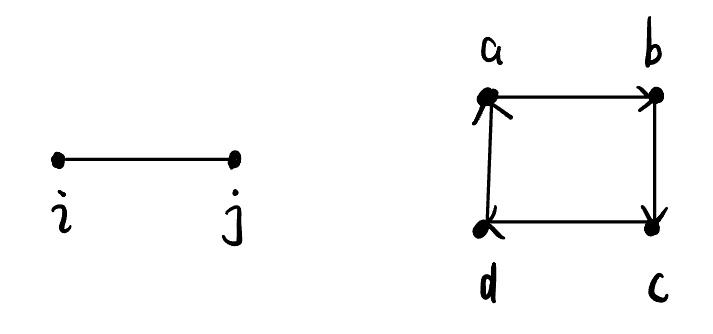
\includegraphics[width=0.35\linewidth]{images/period-2.jpg}
        \caption{左：无向二部图；右：有向环}
        \label{srr-fig:period-1}
    \end{figure}

    举例：图 \ref{srr-fig:period-1}（左）中状态$i$的周期为$\textup{gcd}\{2,4,6,8,\dots\}=2$，因此$i$的周期为$2$；类似地，$j$的周期也为$2$。
        
    \begin{definition}[非周期性]
        \label{defn:aperiodicity}
        若状态$i$的周期为$1$，则状态$i$是非周期性的（aperiodic）。若马尔可夫链中所有的状态都是非周期性的，则这个马尔科夫链是非周期性的。
    \end{definition}

    \textbf{关于周期性的更多例子}
    \begin{itemize}
        \item 无向二部图中状态（即图中顶点）的周期为$2$，例如图 \ref{srr-fig:period-1}（左）；
        \item 长为$k>1$的有向环中点的周期为$k$，例如图 \ref{srr-fig:period-1}（右）；
        \item 周期性阻止概率分布收敛到单一极限分布：
        \begin{itemize}
            \item 例如图 \ref{srr-fig:period-1}（左）中初始状态为$i$的马尔科夫链，奇数步后在$j$，偶数步后在$i$，因此概率分布会在两个分布之间振荡，无法收敛到单一极限。
        \end{itemize}
    \end{itemize}

    \begin{proposition}[可达性结果（Reachability Result）]
        \label{proposition:re-re}
        在任意有限（状态集合有限）、不可约、非周期的马尔可夫链中，存在$\tau<\infty$满足对于所有的$i,j$和$t\ge \tau$有：
        \[
            \Pr[X_t=j\mid X_0=i]>0.
        \]
    \end{proposition}

    注意：仅仅有限、不可约这两个条件不能得出性质 \ref{proposition:re-re} 中的结果。例如针对图 \ref{srr-fig:period-1}（左），其满足有限和不可约，但在$t$为奇数时，$\Pr[X_t=i|X_0=i]=0$，在$t$为偶数时，$\Pr[X_t=j|X_0=i]=0$。即因为周期性，导致某些时刻概率恒为$0$，不满足性质 \ref{proposition:re-re} 中的结果，因此需要“非周期”这个条件。



    \subsubsection{马尔科夫链基本定理}
        
    \begin{definition}[稳态分布]
        \label{defn:stationary-distribution}
        一个概率向量$\vec{\pi}\in\mathbb{R}^n$对于$P$是稳态分布（stationary distribution），如果满足：$\vec{\pi}P=\vec{\pi}$。
    \end{definition}

    \begin{itemize}
        \item $\vec{\pi}$是$P$的左特征向量，对应的特征值为$1$；
        \item 如果$\vec{\pi}$是稳态分布，那么对于所有的$t>0$有$\vec{\pi}P^t=\vec{\pi}$：
        \begin{itemize}
            \item $\vec{\pi}P^t=\vec{\pi}P\cdot P^{t-1}=\vec{\pi}P^{t-1}=\vec{\pi}P\cdot P^{t-2}=\vec{\pi}P^{t-2}=\cdots=\vec{\pi}$。
        \end{itemize}
    \end{itemize}

    \begin{definition}[TV距离]
        \label{defn:tv-distance}
        两个概率分布$\vec{p},\vec{q}\in\mathbb{R}^n$之间的TV距离（total variation distance）定义为
        \[
            d_{\textup{TV}}(\vec{p},\vec{q}):=\frac{1}{2}\sum_{i=1}^n{|p(i)-q(i)|}=\frac{1}{2}\lVert \vec{p}-\vec{q}\rVert_1.
        \]
    \end{definition}

    如果在$t\rightarrow \infty$时有$d_{\textup{TV}}(\vec{p}_t,\vec{q})\rightarrow 0$，则称$\vec{p}_t$（定义 \ref{defn:probability-distribution}）收敛于$\vec{q}$。

    \begin{theorem}[马尔科夫链基本定理] 
        \label{thrm:fund-mc}
        令$P\in \mathbb{R}^{n\times n}$定义一个有限、不可约、非周期的马尔科夫链。则对任意的初始分布$\vec{p}_0$，其对应的$\vec{p}_t:=\vec{p}_0P^t$在$t\rightarrow \infty$时收敛于一个唯一的稳态分布$\vec{\pi}$。
    \end{theorem}

    定理 \ref{thrm:fund-mc} 针对所有满足有限、不可约、非周期的马尔科夫链成立，而无向图上的随机游走是特殊的马尔科夫链，接下来我们运用谱分析证明一个特殊版本（关于无向图上的随机游走）的马尔可夫链基本定理。


        
\subsection{无向图上的简单随机游走}
        
本节我们考虑无向图上的随机游走，这是一种特殊的马尔科夫链，希望运用谱图论证明定理 \ref{thrm:fund-mc}。

\textbf{一些基础符号。}针对无权无向图$G=(V,E)$，$A\in\mathbb{R}^{n\times n}$表示图$G$的邻接矩阵，$D\in\mathbb{R}^{n\times n}$表示度数对角矩阵，其中$D_{ii}=\textup{deg}(i)$。

\vspace{0.2cm}
回忆无权无向图$G=(V,E)$上的随机游走是指从图中某个点出发，在每一步，从当前所在点的邻居中均匀随机地选择一个点进行移动（游走）。
        
\begin{itemize}
    \item 令$P_{ij}$表示从点$i$到点$j$的单步转移概率，则：
    \begin{itemize}
        \item 若$(i,j)\in E$，有$P_{ij}=\frac{1}{\textup{deg}(i)}$；
        \item 若$(i,j)\notin E$，有$P_{ij}=0$；
    \end{itemize}
    \item 因此\textcolor{blue}{转移矩阵$P=D^{-1}A$}。这称为图上简单随机游走的转移矩阵。
    \item 令$\bm{p}_0:V\rightarrow \mathbb{R}$表示初始概率分布，则$\bm{p}_{t+1} = \bm{p}_t P= \bm{p}_t D^{-1}A
        \quad \Rightarrow \quad
        \textcolor{blue}{\bm{p}_t = \bm{p}_0 (D^{-1}A)^t}.$
\end{itemize}

\vspace{0.2cm}
类似定义 \ref{defn:stationary-distribution}，我们定义$\bm{\pi}:V\to \mathbb{R}$为稳态分布，如果$\bm{\pi}$满足$\bm{\pi}P=\bm{\pi}$。$\bm{\pi}$是$P$的左特征向量，对应的特征值为$1$。%针对$P=D^{-1}A$，一个自然的稳态分布$\bm{\pi}$可以定义为$\bm{\pi}(i)=\frac{\textup{deg}(i)}{2|E|}$。

\begin{lemma}
    \label{lemma:sta-dist-graoh}
    令$G=(V,E)$表示一个无向图，令$P=D^{-1}A$。对所有$i\in V$，定义
    \[
        \bm{\pi}(i)=\frac{\textup{deg}(i)}{2|E|},
    \]
    则$\bm{\pi}$是$P$的一个稳态分布。
            
    \begin{proof}
        \begin{align*}
            \bm{\pi}P&=\bm{\pi}D^{-1}A\\
            &=\frac{1}{2|E|}\vec{1}\cdot  A\\
            &=\frac{1}{2|E|}\left(\textup{deg}(1),\dots,\textup{deg}(n)\right)\\
            &=\bm{\pi}.
        \end{align*}
    \end{proof}
\end{lemma}

定理 \ref{thrm:fund-mc} 中马尔科夫链需要满足有限、不可约、非周期三个条件。因此我们需要在图上对应有限、不可约、非周期三个条件。

\paragraph{有限。}只要图上的顶点数$|V|$有限就满足了“有限”这个条件。

\paragraph{不可约。}若$G$是不连通的，则随机游走的长期表现（long-term behavior）取决于起始点，稳态分布也不是唯一的。
        
考虑图$G$中有两个连通分量$G_1=(V_1,E_1)$和$G_2=(V-V_1,E-E_1)$：
\begin{itemize}
    \item 若起始点为$G_1$中的点（即$V_1$中的点），则稳态分布为
    \begin{itemize}
        \item 对$i\in V_1$，$\bm{\pi}(i)=\frac{\textup{deg}(i)}{2|E_1|}$；
        \item 对$i\notin V_1$，$\bm{\pi}(i)=0$；
    \end{itemize}

    \item 若起始点为$G_2$中的点（即$V-V_1$中的点），则稳态分布为
    \begin{itemize}
        \item 对$i\notin V_1$，$\bm{\pi}(i)=\frac{\textup{deg}(i)}{2|E-E_1|}$；
        \item 对$i\in V_1$，$\bm{\pi}(i)=0$。
    \end{itemize}
\end{itemize}

\begin{fact}
    \label{fact:irre-graph}
    当且仅当$G$连通时，不可约条件满足。
\end{fact}

\paragraph{非周期。}即使在连通图中，随机游走也可能不会收敛到一个稳态分布，例如图 \ref{srr-fig:period-1} （左）中的连通二部图，其概率分布会在两个分布之间振荡，无法收敛到单一极限。

\begin{fact}
    \label{fact:aper-graph}
    当且仅当$G$是非二部图（non-bipartite）时，非周期条件满足。
\end{fact}



    \subsubsection{特殊的马尔科夫链基本定理}
        
    结合事实 \ref{fact:irre-graph}、事实 \ref{fact:aper-graph} 和引理 \ref{lemma:sta-dist-graoh}，我们想要证明的特殊版本的定理 \ref{thrm:fund-mc} 变为以下定理：

    \begin{theorem}
        \label{thrm:special-fund-mc}
        令$G$表示一个无向、连通的非二部图，并且转移矩阵$P=D^{-1}A$，则满足以下定义的分布$\bm{\pi}$是\textbf{唯一}的稳态分布：
        \[
            \bm{\pi}(i)=\frac{\textup{deg}(i)}{2|E|}.
        \]
        即对任意的初始分布$\bm{p}_0$，其对应的$\bm{p}_t=\bm{p}_0P^t$在$t\to \infty$时收敛于$\bm{\pi}$%，即$\bm{p}_t=\bm{p}_0P^t\to \bm{\pi}$
            。
    \end{theorem}
        


\subsection{$d$-正则非二部图上的简单随机游走}

    接下来我们的目标是使用\textbf{谱分析（spectral analysis）}证明上节中给出的特殊的马尔可夫链基本定理（定理 \ref{thrm:special-fund-mc}），即证明随机游走会收敛到一个唯一的稳态分布。此外谱技巧（spectral techniques）可以精确分析混合时间（mixing time），即收敛速度。 本节首先考虑在一类特殊的图（$d$-正则非二分图）上进行证明，在后面章节推广到更一般的图上。

    对$d$-正则图：
    \begin{itemize}
        \item 简单随机游走的转移矩阵$P=D^{-1}A=\frac{1}{d}A=\mathcal{A}$；
        \begin{itemize}
            \item $\mathcal{A}$为正则化的邻接矩阵；
        \end{itemize}
        \item $P$为实对称矩阵，因此特征值都是实数；
        \item 稳态分布满足$\bm{\pi}(i)=\frac{d}{dn}=\frac{1}{n}$，因此$\bm{\pi}=\frac{\bm{1}}{n}$。
    \end{itemize}

    \vspace{0.2cm}
    \textbf{$P=\mathcal{A}$的谱性质。}令$\alpha_1\ge \alpha_2\ge \dots\ge \alpha_n$表示$\mathcal{A}$的特征值，对应的一组标准正交特征向量为$v_1,v_2,\dots,v_n$：
    \begin{itemize}
        \item 由Notes Lec 10中引理 28 可知，$\alpha_1=1$，且$v_1=\frac{\bm{1}}{\sqrt{n}}$；
        \item \textcolor{blue}{当且仅当$G$是连通图时，$\alpha_2<1$}；
            \begin{itemize}
                \item 由Notes Lec 10中引理 22 可知，当且仅当$G$是连通图时，$L=D-A$的第二小特征值$\lambda_2>0$（对应的特征向量为$v_2$），可以验证$\alpha_i=1-\frac{\lambda_i}{d}$，因此$\alpha_2=1-\frac{\lambda_2}{d}<1$；
            \end{itemize}
        \item \textcolor{blue}{当且仅当$G$是非二部图时，$\alpha_n>-1$}（当且仅当$G$是二部图时，$\alpha_n=-1$）；
            \begin{itemize}
                \item 由Notes Lec 10中引理 12 可得。
            \end{itemize}
        \end{itemize}

    \vspace{0.25cm}
    下面给出与定理 \ref{thrm:special-fund-mc} 相对应的$d$-正则非二部图上的结论，即定理 \ref{thrm:fund-mc-d-1}。
            
    \begin{theorem}
        \label{thrm:fund-mc-d-1}
        令$G$表示一个$d$-正则化的、无向、连通的非二部图，简单随机游走的转移矩阵$P=D^{-1}A=\mathcal{A}$，那么对于所有的初始概率分布$\bm{p}_0$：
        \[
            \lim_{t \to \infty} \bm{p}_0\mathcal{A}^t  = \frac{\bm{1}}{n}.
        \]
    \end{theorem}

    \begin{proof}
        % 因为$\mathcal{A}$的特征向量$v_1,\dots,v_n$构成一组标准正交基，因此任意的初始向量$\bm{p}_0$都可以用$v_1,\dots,v_n$表示，即$\bm{p}_0=\sum_{i=1}^n{c_iv_i^{\top}}$，其中$c_1,\dots,c_n$为常数。
                    
        % 此外，
        $\mathcal{A}$的特征分解可以表示为$\mathcal{A}=\sum_{i=1}^n{\alpha_iv_iv_i^{\top}}$。由于$v_1,\dots,v_n$构成一组标准正交基，则对任意$i\ne j$有$v_i^{\top}v_j=0$，对任意$i\in[n]$有$v_i^{\top}v_i=1$。因此$\mathcal{A}^t=\sum_{i=1}^n{\alpha_i^tv_iv_i^{\top}}$。

        \begin{align*}
            \bm{p}_0\mathcal{A}^t&=\bm{p}_0\sum_{i=1}^n{\alpha_i^tv_iv_i^{\top}}\\
            &=\bm{p}_0\cdot \alpha_1^tv_1v_1^{\top}+\bm{p}_0\sum_{i=2}^n{\alpha_i^tv_iv_i^{\top}}\\
            &=\frac{\bm{1}}{n}+\bm{p}_0\sum_{i=2}^n{\alpha_i^tv_iv_i^{\top}}&&\text{（$\alpha_1=1,v_1=\frac{\bm{1}}{\sqrt{n}}$且$\bm{p}_0$满足$\sum_{i=1}^n\bm{p}_0(i)=1$）}
        \end{align*}

        等式两边同时取极限，可得：
                    
        \begin{align*}
            \lim_t \bm{p}_0\mathcal{A}^t =\lim_t \frac{\bm{1}}{n}+\bm{p}_0\sum_{i=2}^n{\alpha_i^tv_iv_i^{\top}}=\frac{\bm{1}}{n},
        \end{align*}
        
        这是因为在连通的非二部图中，$1>\alpha_2\ge \alpha_3\ge \dots\ge \alpha_n>-1$，因此在$t\to \infty$时，$\forall i>1$，${|\alpha_i^t|}\to 0$，即$\bm{p}_0\sum_{i=2}^n{\alpha_i^tv_iv_i^{\top}}\to 0$。
                    
    \end{proof}

    马尔科夫链基本定理表明在步数$t\to \infty$时，随机游走的概率分布趋于稳态分布。现在我们关心$t$足够大时，随机游走概率分布的表现，而不是$t\to \infty$时。因此我们引入混合时间（mixing time）的概念。

    \begin{definition}[混合时间]
        \label{defn:mixing-time}
        对于转移矩阵为$P$的随机游走，令$\bm{p}_t=\bm{p}_0P^t$表示从初始分布$\bm{p}_0$开始的步长为$t$的随机游走的概率分布，$\bm{\pi}=\lim_{t \to \infty} \bm{p}_t$表示稳态分布。混合时间$\tau_{\varepsilon}(P)$定义为对任意初始分布$\bm{p}_0$，满足$d_{\textup{TV}}(\bm{p}_t,\bm{\pi})\le \varepsilon$的最小的步数$t$。
    \end{definition}

    在本节中，除非$\varepsilon$被特殊指明，否则我们默认$\varepsilon=1/4$。接下来我们给出简单随机游走混合时间的上界。%与上节类似，我们首先在一类特殊的图（$d$-正则图）上给出混合时间的上界（更简单），其次在更一般的图上给出混合时间的上界。

    回忆在$d$-正则图上，$P=D^{-1}A=\frac{1}{d}A=\mathcal{A}$，$W=\frac{1}{2}I+\frac{1}{2}P=\frac{1}{2}I+\frac{1}{2}\mathcal{A}$。$1=\alpha_1\ge \alpha_2\ge\dots \ge \alpha_n\ge -1$表示$\mathcal{A}$的特征值，对应的一组标准正交的特征向量为$v_1,\dots,v_n$。稳态分布为$\bm{\pi}=\frac{\bm{1}}{n}$。

    定义\textbf{谱间隔（spectral gap）}为$g:=\min\{1-\alpha_2,1-|\alpha_n|\}$。

    \paragraph{通过谱间隔给出混合时间的上界：}

    \begin{fact}
        \label{fact:norm}
        对任意向量$x\in\mathbb{R}^n$，有$\lVert x\rVert_1\le \sqrt{n}\lVert x\rVert_2$。
        \begin{proof}
            利用柯西不等式：
            \begin{align*}
                \lVert x\rVert_1=\sum_{i=1}^n{|x(i)|}
                \le \sqrt{\left(\sum_{i=1}^n{1^2}\right)\left(\sum_{i=1}^n{x(i)^2}\right)}
                =\sqrt{n}\cdot \lVert x\rVert_2.
            \end{align*}
        \end{proof}
    \end{fact}
                
    \begin{theorem}
        \label{thrm:mixing-time-d-sg}
        令$G$表示一个无向、连通、非二部图的$d$-正则图，$P=\mathcal{A}$为图上的简单随机游走转移矩阵。则$\tau_{\varepsilon}(P)\lesssim\frac{1}{g}\ln{\left(\frac{n}{\varepsilon}\right)}$。
    \end{theorem}

    注：$a \lesssim b$中$\lesssim$符号隐藏了常数，表示$a\le c\cdot b$，其中$c$是一个常数。可以认为$\lesssim$符号与$O$符号类似。

    定理 \ref{thrm:mixing-time-d-sg} 表明无向、连通、非二部图（连通的非二部图的$g>0$）的$d$-正则图上简单随机游走的混合时间与谱间隔$g$有关。

    \begin{proof}
        因为$\mathcal{A}$的特征向量$v_1,\dots,v_n$（列向量）构成一组标准正交基，因此任意的初始向量$\bm{p}_0$（行向量）都可以用$v_1,\dots,v_n$表示，即$\bm{p}_0=\sum_{i=1}^n{c_iv_i^{\top}}$，其中$c_1,\dots,c_n$为常数。此外，$P=\mathcal{A}=\sum_{i=1}^n{\alpha_iv_iv_i^{\top}}$，且$P^t=\mathcal{A}^t=\sum_{i=1}^n{\alpha_i^tv_iv_i^{\top}}$。%则$\bm{p}_t=\bm{p}_0P^t=\sum_{i=1}^n{c_i\alpha_i^tv_i^{\top}}$。
        
        由定理 \ref{thrm:fund-mc-d-1} 的证明可知$\bm{p}_t=\bm{p}_0P^t=\frac{\bm{1}}{n}+\bm{p}_0\sum_{i=2}^n{\alpha_i^tv_iv_i^{\top}}$，因此
                    
        \begin{align*}
            d_{\textup{TV}}(\bm{p}_t,\bm{\pi})&=\frac{1}{2}\lVert \bm{p}_t-\bm{\pi} \rVert_1\\
            % &\le \lVert \bm{p}_t-\bm{\pi} \rVert_1\\
            &=\frac{1}{2}\lVert \frac{\bm{1}}{n}+\bm{p}_0\sum_{i=2}^n{\alpha_i^tv_iv_i^{\top}}-\frac{\bm{1}}{n}\rVert_1\\
            &=\frac{1}{2}\lVert \bm{p}_0\sum_{i=2}^n{\alpha_i^tv_iv_i^{\top}}\rVert_1\\
            &=\frac{1}{2}\lVert \sum_{i=2}^n{c_i\alpha_i^tv_i^{\top}}\rVert_1&&\text{($\bm{p}_0=\sum_{i=1}^n{c_iv_i^{\top}}$)}\\
            &\le \frac{\sqrt{n}}{2}\lVert \sum_{i=2}^n{c_i\alpha_i^tv_i^{\top}}\rVert_2&&\text{（事实 \ref{fact:norm}）}.
        \end{align*}

        令向量$X=\sum_{i=2}^n{c_i\alpha_i^tv_i^{\top}}$，则$X(k)=\sum_{i=2}^n{c_i\alpha_i^tv_i(k)}$，因此
        
        \begin{align*}
            \lVert \sum_{i=2}^n{c_i\alpha_i^tv_i^{\top}}\rVert_2^2&=\lVert X\rVert_2^2\\
            &=\sum_{k=1}^n{X(k)^2}\\
            &=\sum_{k=1}^n{\left(\sum_{i=2}^n{c_i\alpha_i^tv_i(k)}\right)^2}\\
            &=\sum_{k=1}^n{\left(\sum_{i=2}^n{\sum_{j=2}^n{c_i\alpha_i^tv_i(k)\cdot c_j\alpha_j^tv_j(k)}}\right)}\\
            &=\sum_{i=2}^n{\sum_{j=2}^n{c_i\alpha_i^tc_j\alpha_j^t\sum_{k=1}^n{v_i(k)v_j(k)}}}\\
            &=\sum_{i=2}^n{c_i^2\alpha_i^{2t}}&&\text{（$v_1,\dots,v_n$是一组标准正交基）}\\
            &\le (1-g)^{2t}\sum_{i=2}^n{c_i^2}\\
            &\le e^{-2gt}\sum_{i=2}^n{c_i^2}.
        \end{align*}

        结合上面两个式子，有：
        
        \begin{align*}
            d_{\textup{TV}}(\bm{p}_t,\bm{\pi})&\le \frac{\sqrt{n}}{2}\lVert \sum_{i=2}^n{c_i\alpha_i^tv_i^{\top}}\rVert_2\\
            &\le\frac{\sqrt{n}}{2}\sqrt{e^{-2gt}\sum_{i=2}^n{c_i^2}}\\
            &\le\frac{\sqrt{n}}{2}\sqrt{e^{-2gt}\sum_{i=1}^n{c_i^2}}\\
            &=\frac{\sqrt{n}}{2}\sqrt{e^{-2gt}\left\|p_0\right\|_2^2}\\
            &\le\frac{\sqrt{n}}{2}\sqrt{e^{-2gt}\left\|p_0\right\|_1}\\
            &=\frac{\sqrt{n}}{2}e^{-gt}\\
            &=\frac{\sqrt{n}}{2}e^{-g\cdot C\frac{1}{g}\ln{\left(\frac{n}{\varepsilon}\right)}}&&\text{（$t=\tau_{\varepsilon}(P)\lesssim\frac{1}{g}\ln{\left(\frac{n}{\varepsilon}\right)}$）}\\
            &=\frac{\sqrt{n}}{2}\left(\frac{\varepsilon}{n}\right)^{C}\\
            &\le \varepsilon.&&\text{（取足够大的$C\ge 1$）}\\
            %&\lesssim \sqrt{n}e^{-tg}.
        \end{align*}
    \end{proof}

    

            
\subsection{$d$-正则图上的懒惰随机游走}

\paragraph{去掉非周期性条件。}定理 \ref{thrm:special-fund-mc} 中的非二部图保证了马尔可夫链是非周期的（事实 \ref{fact:aper-graph}）。若想移除非二部图这个条件，我们可以给图上的点加自环（self-loops）。这将引出懒惰随机游走（lazy random walk）的概念。本节中我们首先研究$d$-正则非二分图上的懒惰随机游走。

\begin{definition}[（$d$-正则图上的）懒惰随机游走]
    \label{defn:lazy-random-walk-regular}
    给定一个$d$-正则无向图$G$，其上的懒惰随机游走对应的转移矩阵$W$定义为：\[W=\frac{1}{2}I+\frac{A}{2d}.\]
\end{definition}

直观上看，图上的懒惰随机游走从某个点开始，在每一步，以$\frac{1}{2}$的概率留在原地，以$\frac{1}{2}$的概率随机均匀随机地选择一个邻居进行转移（游走）。

考虑懒惰随机游走的好处：
\begin{itemize}
    \item 加自环打破了二部图的周期性；
    \item 这种修改确保马尔可夫链变为非周期性的，同时不会显著改变图的结构。
\end{itemize}

\iffalse
\begin{corollary}
    \label{coro:fund-mc-lazy}
    令$G$表示一个无向、连通图。令$W=\frac{1}{2}I+\frac{1}{2}D^{-1}A$表示懒惰随机游走的转移矩阵。则满足以下定义的分布$\bm{\pi}$是\textbf{唯一}的稳态分布：
    \[
        \bm{\pi}(i)=\frac{\textup{deg}(i)}{2|E|}.
    \]
    即对任意的初始分布$\bm{p}_0$，其对应的$\bm{p}_t=\bm{p}_0W^t$在$t\to \infty$时收敛于$\bm{\pi}$%，即$\bm{p}_t=\bm{p}_0W^t\to \bm{\pi}$
    。
\end{corollary}
\fi

首先分析懒惰随机游走转移矩阵$W$的谱性质。
            
\vspace{0.2cm}
\textbf{$W$的谱性质。}由$W=\frac{1}{2}I+\frac{1}{2}\mathcal{A}$可知，$W$的特征值为$\frac{1}{2}(1+\alpha_i)$，对应的特征向量为$v_i$。$W$的特征值$\frac{1}{2}(1+\alpha_i)$有以下规律：
\begin{itemize}
    \item $W$的最大特征值为$\frac{1}{2}(1+\alpha_1)=1$；
    \item 因为$\alpha_i\ge -1$，因此对所有$i\in[n]$，$W$的特征值$\frac{1}{2}(1+\alpha_i)\ge 0$；
    \item $1> \frac{1+\alpha_2}{2}\ge \dots\ge \frac{1+\alpha_n}{2}\ge 0$。
\end{itemize}
            
下面给出$d$-正则非二分图上的稳态分布，即定理 \ref{thrm:fund-mc-d-2}。

\begin{theorem}
    \label{thrm:fund-mc-d-2}
    令$G$表示一个$d$-正则化的、无向、连通图，转移矩阵$W=\frac{1}{2}I+\frac{1}{2}\mathcal{A}$，那么对于所有的初始概率分布$\bm{p}_0$：
    \[
        \lim_{t \to \infty} \bm{p}_0W^t  = \frac{\bm{1}}{n}.
    \]
\end{theorem}

\begin{proof}
    （证明与定理 \ref{thrm:fund-mc-d-1} 类似。）由$W$的谱性质可知，$W$的特征值为$\frac{1}{2}(1+\alpha_i)$，对应的特征向量为$v_i$，因此$W$的特征分解可以表示为$W=\sum_{i=1}^n{\frac{1+\alpha_i}{2}v_iv_i^{\top}}$，类似地，$W^t=\sum_{i=1}^n{\left(\frac{1+\alpha_i}{2}\right)^tv_iv_i^{\top}}$。
    \begin{align*}
        \bm{p}_0W^t&=\bm{p}_0\sum_{i=1}^n{\left(\frac{1+\alpha_i}{2}\right)^tv_iv_i^{\top}}\\
        &=\bm{p}_0\left(\frac{1+\alpha_1}{2}\right)v_1v_1^{\top}+\bm{p}_0\sum_{i=2}^n{\left(\frac{1+\alpha_i}{2}\right)^tv_iv_i^{\top}}\\
        &=\frac{\bm{1}}{n}+\bm{p}_0\sum_{i=2}^n{\left(\frac{1+\alpha_i}{2}\right)^tv_iv_i^{\top}}&&\text{（$\alpha_1=1,v_1=\frac{\bm{1}}{\sqrt{n}}$且$\bm{p}_0$满足$\sum_{i=1}^n\bm{p}_0(i)=1$）}
    \end{align*}

    等式两边同时取极限，可得：
    \begin{align*}
        \lim_t \bm{p}_0W^t =\lim_t \left(\frac{\bm{1}}{n}+\bm{p}_0\sum_{i=2}^n{\left(\frac{1+\alpha_i}{2}\right)^tv_iv_i^{\top}}\right)=\frac{\bm{1}}{n},
    \end{align*}
    
    这是因为在连通图中，$1>\alpha_2\ge \alpha_3\ge \dots\ge \alpha_n>-1$，因此$1> \frac{1+\alpha_2}{2}\ge \dots\ge \frac{1+\alpha_n}{2}\ge 0$。则在$t\to \infty$时，$\forall i>1$，${|\left(\frac{1+\alpha_i}{2}\right)^t|}\to 0$，即$\bm{p}_0\sum_{i=2}^n{\left(\frac{1+\alpha_i}{2}\right)^tv_iv_i^{\top}}\to 0$。
\end{proof}

\paragraph{通过导率（conductance）给出混合时间的上界：}
                
回忆在$d$-正则图上，懒惰随机游走的转移矩阵$W=\frac{1}{2}I+\frac{1}{2}P=\frac{1}{2}I+\frac{1}{2}\mathcal{A}$，$W$的特征值为$\frac{1}{2}(1+\alpha_i)$，均$\ge 0$。稳态分布为$\bm{\pi}=\frac{\bm{1}}{n}$。此外，图$G$的正则化拉普拉斯矩阵$\mathcal{L}=I-\frac{A}{d}=I-\mathcal{A}$，特征值为$0\le\lambda_1\le \lambda_2\le\dots\le \lambda_n\le 2$（对应的特征向量为$v_1,\dots,v_n$），其中$\lambda_i=1-\alpha_i$。

定义\textbf{谱间隔（spectral gap）}为$g:=\frac{1}{2}(1-\alpha_2)=\frac{1}{2}\lambda_2$。

\begin{theorem}
    \label{thrm:mixing-time-d-c}
    令$G$表示一个无向、连通的$d$-正则图，$W=\frac{1}{2}I+\frac{1}{2}\mathcal{A}$为图上的懒惰随机游走转移矩阵。则$\tau_{\varepsilon}(W)\lesssim\frac{1}{\phi(G)^2}\ln{\left(\frac{n}{\varepsilon}\right)}$。
\end{theorem}

定理 \ref{thrm:mixing-time-d-c} 表明无向、连通（连通图的$g>0$，即$\phi(G)>0$）的$d$-正则图上懒惰随机游走的混合时间与导率$\phi(G)$有关。

\begin{proof}
    （总体证明思路与定理 \ref{thrm:mixing-time-d-sg} 的证明类似，最后用到Cheeger不等式。）

    由定理 \ref{thrm:fund-mc-d-2} 的证明可知$\bm{p}_t=\bm{p}_0W^t=\frac{\bm{1}}{n}+\bm{p}_0\sum_{i=2}^n{\left(\frac{1+\alpha_i}{2}\right)^tv_iv_i^{\top}}$，因此

    \[
        d_{\textup{TV}}(\bm{p}_t,\bm{\pi})\le \frac{\sqrt{n}}{2}\lVert \sum_{i=2}^n{c_i\left(\frac{1+\alpha_i}{2}\right)^tv_i^{\top}}\rVert_2.
    \]
                    % \begin{align*}
                    %     d_{\textup{TV}}(\bm{p}_t,\bm{\pi})&=\frac{1}{2}\lVert \bm{p}_t-\bm{\pi} \rVert_1\\
                    %     % &\le \lVert \bm{p}_t-\bm{\pi} \rVert_1\\
                    %     &=\frac{1}{2}\lVert \frac{\bm{1}}{n}+\bm{p}_0\sum_{i=2}^n{\left(\frac{1+\alpha_i}{2}\right)^tv_iv_i^{\top}}-\frac{\bm{1}}{n}\rVert_1\\
                    %     &=\frac{1}{2}\lVert \bm{p}_0\sum_{i=2}^n{\left(\frac{1+\alpha_i}{2}\right)^tv_iv_i^{\top}}\rVert_1\\
                    %     &=\frac{1}{2}\lVert \sum_{i=2}^n{c_i\left(\frac{1+\alpha_i}{2}\right)^tv_i^{\top}}\rVert_1&&\text{($\bm{p}_0=\sum_{i=1}^n{c_iv_i^{\top}}$)}\\
                    %     &\le \frac{\sqrt{n}}{2}\lVert \sum_{i=2}^n{c_i\left(\frac{1+\alpha_i}{2}\right)^tv_i^{\top}}\rVert_2&&\text{（事实 \ref{fact:norm}）}.
                    % \end{align*}

    此外，
    
    \begin{align*}
        \lVert \sum_{i=2}^n{c_i\left(\frac{1+\alpha_i}{2}\right)^tv_i^{\top}}\rVert_2^2&=\sum_{i=2}^n{c_i^2\left(\frac{1+\alpha_i}{2}\right)^{2t}}\\
        &=\sum_{i=2}^n{c_i^2\left(1-\frac{\lambda_i}{2}\right)^{2t}}&&\text{（$\lambda_i=1-\alpha_i$）}\\
        &\le (1-g)^{2t}\sum_{i=1}^n{c_i^2}\\
        &\le e^{-2gt}\sum_{i=2}^n{c_i^2}.
    \end{align*}
                    % 令向量$X=\sum_{i=2}^n{c_i\left(\frac{1+\alpha_i}{2}\right)^tv_i^{\top}}$，则$X(k)=\sum_{i=2}^n{c_i\left(\frac{1+\alpha_i}{2}\right)^tv_i(k)}$，因此
                    % \begin{align*}
                    %     \lVert \sum_{i=2}^n{c_i\left(\frac{1+\alpha_i}{2}\right)^tv_i^{\top}}\rVert_2^2&=\lVert X\rVert_2^2\\
                    %     &=\sum_{k=1}^n{X(k)^2}\\
                    %     &=\sum_{k=1}^n{\left(\sum_{i=2}^n{c_i\left(\frac{1+\alpha_i}{2}\right)^tv_i(k)}\right)^2}\\
                    %     &=\sum_{k=1}^n{\left(\sum_{i=2}^n{\sum_{j=2}^n{c_i\left(\frac{1+\alpha_i}{2}\right)^tv_i(k)\cdot c_j\left(\frac{1+\alpha_j}{2}\right)^tv_j(k)}}\right)}\\
                    %     &=\sum_{i=2}^n{\sum_{j=2}^n{c_i\left(\frac{1+\alpha_i}{2}\right)^tc_j\left(\frac{1+\alpha_j}{2}\right)^t\sum_{k=1}^n{v_i(k)v_j(k)}}}\\
                    %     &=\sum_{i=2}^n{c_i^2\left(\frac{1+\alpha_i}{2}\right)^{2t}}&&\text{（$v_1,\dots,v_n$是一组标准正交基）}\\
                    %     &\le (1-g)^{2t}\sum_{i=2}^n{c_i^2}\\
                    %     &\le e^{-2gt}\sum_{i=2}^n{c_i^2}.
                    % \end{align*}

    结合上面两个式子，有：
    
    \begin{align*}
        d_{\textup{TV}}(\bm{p}_t,\bm{\pi})&\le \frac{\sqrt{n}}{2}\lVert \sum_{i=2}^n{c_i\left(\frac{1+\alpha_i}{2}\right)^tv_i^{\top}}\rVert_2\\
        &\le\frac{\sqrt{n}}{2}\sqrt{e^{-2gt}\sum_{i=2}^n{c_i^2}}\\
        &\le\frac{\sqrt{n}}{2}\sqrt{e^{-2gt}\sum_{i=1}^n{c_i^2}}\\
            &=\frac{\sqrt{n}}{2}\sqrt{e^{-2gt}\left\|p_0\right\|_2^2}\\
            &\le\frac{\sqrt{n}}{2}\sqrt{e^{-2gt}\left\|p_0\right\|_1}\\
            &=\frac{\sqrt{n}}{2}e^{-gt}\\
            &=\frac{\sqrt{n}}{2}e^{-g\cdot C\frac{1}{g}\ln{\left(\frac{n}{\varepsilon}\right)}}&&\text{（$t=\tau_{\varepsilon}(P)\lesssim\frac{1}{g}\ln{\left(\frac{n}{\varepsilon}\right)}$）}\\
            &=\frac{\sqrt{n}}{2}\left(\frac{\varepsilon}{n}\right)^{C}\\
            &\le \varepsilon.&&\text{（取足够大的$C\ge 1$）}\\
        %&\lesssim \sqrt{n}e^{-tg}.
    \end{align*}
                    
    由Notes Lec 14中的Cheeger不等式可知$\frac{\lambda_2}{2}\le \phi(G)\le \sqrt{2\lambda_2}$，因此$\lambda_2\ge \frac{\phi(G)^2}{2}$，$g=\frac{1}{2}\lambda_2\ge \frac{\phi(G)^2}{4}$，因此$\tau_{\varepsilon}(W)\le C_2\frac{1}{g}\ln{\left(\frac{n}{\varepsilon}\right)}\le 4C_2 \frac{1}{\phi(G)^2}\ln{\left(\frac{n}{\varepsilon}\right)}$，即$\tau_{\varepsilon}(W)\lesssim  \frac{1}{\phi(G)^2}\ln{\left(\frac{n}{\varepsilon}\right)}$。
\end{proof}

\textbf{应用：}对于扩展图（expanders）$G$，其导率满足$\phi(G)=\Omega(1)$，根据定理 \ref{thrm:mixing-time-d-c}，扩展图上的混合时间为$\tau_{\varepsilon}(W)=O(\log n)$，这一结论在以下场景下有用：
    \begin{itemize}
        \item 均匀采样；
        \item 设计随机化算法（randomized algorithms）；
        \item 快速混合马尔科夫链。
    \end{itemize}

总结：通过给图加自环、分析新图上懒惰随机游走可以简化分析。此外，加自环不会显著影响图上随机游走的性质。

            


\subsection{一般非二部图上的简单随机游走}

本节我们首先证明一般图上的马尔科夫链基本定理。其次给出一般图上的混合时间的上界。我们依然首先关心非二部图的情况。

\vspace{0.2cm}
对一般图：
\begin{itemize}
    \item 简单随机游走的转移矩阵$P=D^{-1}A$；
    \item 由于图不一定是$d$-正则图，因此$P$不一定是对称矩阵；
    \begin{itemize}
        \item 因此，谱定理（Notes Lec 10中的定理3）无法直接应用。
    \end{itemize}
\end{itemize}

\vspace{0.2cm}
\textbf{谱的相似性（spectral similarity）：}两个矩阵在谱性质上相似通常指它们的特征值/特征向量可以通过某种方式一一对应，且谱性质相近。如果两个矩阵$M,N$相似，即存在可逆矩阵$S$满足$M=S^{-1}NS$，则$M,N$具有相同的特征值（但特征向量可能不同）。
            
\vspace{0.2cm}
定义正则化邻接矩阵$\mathcal{A}=D^{-1/2}AD^{-1/2}$，可以验证$\mathcal{A}$一定为实对称矩阵。此时：
\begin{itemize}
    \item $P=D^{-1}A=D^{-1/2}\mathcal{A}D^{1/2}$，与$\mathcal{A}$相似，记为$P\sim \mathcal{A}$
    \item 根据谱的相似性，$P$的特征值与$\mathcal{A}$的特征值相同，均为实数。
\end{itemize}

\begin{lemma}
    \label{lemma:similarity-P}
    令$G$表示一个连通的无向图，其正则化邻接矩阵为$\mathcal{A}$。令$\alpha_1>\alpha_2\ge \dots\ge \alpha_n$表示$\mathcal{A}$的特征值，对应的一组标准正交特征向量为$v_1,\dots,v_n$，其中$v_1=\frac{1}{\sqrt{2|E|}}D^{1/2}\bm{1}$。
    则：
    \begin{itemize}
        \item $P=D^{-1}A$的特征值为$\alpha_1,\dots,\alpha_n$；
        \item $P$的特征向量为$D^{-1/2}v_1,\dots,D^{-1/2}v_n$。
    \end{itemize}
\end{lemma}

\begin{proof}
    利用谱的相似性依次证明：
    \begin{itemize}
        \item 由于$P\sim \mathcal{A}$，因此$P$与$\mathcal{A}$的特征值相同，为$\alpha_1,\dots,\alpha_n$；
        \item $PD^{-1/2}v_i=D^{-1/2}\mathcal{A}D^{1/2}D^{-1/2}v_i=D^{-1/2}\mathcal{A}v_i=D^{-1/2}\alpha_iv_i=\alpha_iD^{-1/2}v_i$。
    \end{itemize}
\end{proof}

注意$v_1,\dots,v_n$是一组标准正交基，即对于任意$i\ne j\in[n]$，有$\langle v_i,v_j\rangle=0$；对于任意$i\in[n]$，有$\lVert v_i\rVert_2=\sqrt{v_i^{\top}v_i} =1$。但$P$的特征向量$D^{-1/2}v_1,\dots,D^{-1/2}v_n$不一定是一组标准正交基。因此，我们定义带权重的内积：
\begin{itemize}
    \item $\langle u,v\rangle_{D}=u^{\top}Dv$；
    \item $\lVert v\rVert_{D}=\sqrt{v^{\top}Dv}$。
\end{itemize}

在带权重内积的度量下，$P$的特征向量$D^{-1/2}v_1,\dots,D^{-1/2}v_n$是一组标准正交基，即：
\begin{itemize}
    \item 对于任意$i\ne j\in[n]$，有$\langle D^{-1/2}v_i,D^{-1/2}v_j\rangle_D=0$；
    \item 对于任意$i\in[n]$，有$\Vert D^{-1/2}v_i\rVert_D =1$。
\end{itemize}

\vspace{0.25cm}
下面给出与定理 \ref{thrm:special-fund-mc}、定理 \ref{thrm:fund-mc-d-1} 相对应的一般图上的结论，即定理 \ref{thrm:fund-mc-g-1}。
            
\begin{theorem}
    \label{thrm:fund-mc-g-1}
    令$G$表示一个无向、连通的非二部图，简单随机游走的转移矩阵$P=D^{-1}A=D^{-1/2}\mathcal{A}D^{1/2}$，特征值为$1=\alpha_1>\alpha_2\ge\dots \ge \alpha_n> -1$。那么对于所有的初始概率分布$\bm{p}_0$：
    \[
        \lim_{t \to \infty} \bm{p}_0P^t  = \frac{\bm{d}}{2|E|},
    \]
    其中$\bm{d}\in \mathbb{R}^n,\bm{d}(i)=\textup{deg}(i)$。
\end{theorem}
                
\begin{proof}
    % 因为$\mathcal{A}$的特征向量$v_1,\dots,v_n$构成一组标准正交基，因此任意的初始向量$\bm{p}_0$都可以用$v_1,\dots,v_n$表示，即$\bm{p}_0=\sum_{i=1}^n{c_iv_i^{\top}}$，其中$c_1,\dots,c_n$为常数。
                    
    % 此外，
    因为$P=D^{-1/2}\mathcal{A}D^{1/2}$，因此$P^t=D^{-1/2}\mathcal{A}^tD^{1/2}$。此外，$\mathcal{A}$的特征分解可以表示为$\mathcal{A}=\sum_{i=1}^n{\alpha_iv_iv_i^{\top}}$，$\mathcal{A}^t=\sum_{i=1}^n{\alpha_i^tv_iv_i^{\top}}$，因此$P^t=D^{-1/2}\left(\sum_{i=1}^n{\alpha_i^tv_iv_i^{\top}}\right)D^{1/2}$。
                    
    \begin{align*}
        \bm{p}_0P^t&=\bm{p}_0D^{-1/2}\left(\sum_{i=1}^n{\alpha_i^tv_iv_i^{\top}}\right)D^{1/2}\\
        &=\bm{p}_0\cdot D^{-1/2}\alpha_1^tv_1v_1^{\top}D^{1/2}+\bm{p}_0D^{-1/2}\left(\sum_{i=2}^n{\alpha_i^tv_iv_i^{\top}}\right)D^{1/2}\\
        &=\frac{\bm{d}}{2|E|}+\bm{p}_0D^{-1/2}\left(\sum_{i=2}^n{\alpha_i^tv_iv_i^{\top}}\right)D^{1/2}&&\text{（$\alpha_1=1,v_1=\frac{1}{\sqrt{2|E|}}D^{1/2}\bm{1}$且$\sum_{i=1}^n\bm{p}_0(i)=1$）}
    \end{align*}

    等式两边同时取极限，可得：
                    
    \begin{align*}
        \lim_t \bm{p}_0P^t =\lim_t \left(\frac{\bm{d}}{2|E|}+\bm{p}_0D^{-1/2}\left(\sum_{i=2}^n{\alpha_i^tv_iv_i^{\top}}\right)D^{1/2}\right)=\frac{\bm{d}}{2|E|},
    \end{align*}

    这是因为在连通的非二部图中，$1>\alpha_2\ge \alpha_3\ge \dots\ge \alpha_n>-1$，因此在$t\to \infty$时，$\forall i>1$，${|\alpha_i^t|}\to 0$，即$\bm{p}_0D^{-1/2}\left(\sum_{i=2}^n{\alpha_i^tv_iv_i^{\top}}\right)D^{1/2}\to 0$。
\end{proof}

定义\textbf{谱间隔（spectral gap）}为$g:=\min\{1-\alpha_2,1-|\alpha_n|\}$。

\paragraph{通过谱间隔给出混合时间的上界：}

\begin{theorem}
    \label{thrm:mixing-time-g-sg}
    令$G$表示一个无向、连通的非二部图，$P=D^{-1}A=D^{-1/2}\mathcal{A}D^{1/2}$为图上的简单随机游走转移矩阵。则$\tau_{\varepsilon}(P)\lesssim\frac{1}{g}\ln{\left(\frac{n}{\varepsilon}\right)}$。对于带权的无向、连通、非二部图，$\tau_{\varepsilon}(P)\lesssim\frac{1}{g}\ln{\left(\frac{n}{\varepsilon\cdot \bm{\pi}_{\textup{min}}}\right)}$，其中$\bm{\pi}_{\textup{min}}=\min_{i\in[n]}{\bm{\pi}(i)}=\min_{i\in [n]}{\frac{\textup{deg}(i)}{2|E|}}$。



                % \begin{proof}
                %     因为$\mathcal{A}$的特征向量$v_1,\dots,v_n$（列向量）构成一组标准正交基，因此任意的初始向量$\bm{p}_0$（行向量）都可以用$v_1,\dots,v_n$表示，即$\bm{p}_0=\sum_{i=1}^n{c_iv_i^{\top}}$，其中$c_1,\dots,c_n$为常数。此外，由定理 \ref{thrm:fund-mc-g-1} 的证明可知$\bm{p}_t=\bm{p}_0P^t=\frac{\bm{d}}{2|E|}+\bm{p}_0D^{-1/2}\left(\sum_{i=2}^n{\alpha_i^tv_iv_i^{\top}}\right)D^{1/2}$。

                %     \begin{align*}
                %         d_{\textup{TV}}(\bm{p}_t,\bm{\pi})&=\frac{1}{2}\lVert \bm{p}_t-\bm{\pi} \rVert_1\le \lVert \bm{p}_t-\bm{\pi} \rVert_1\\
                %         % &\le \lVert \bm{p}_t-\bm{\pi} \rVert_1\\
                %         % &=\frac{1}{2}\lVert \frac{\bm{1}}{n}+\bm{p}_0\sum_{i=2}^n{\alpha_i^tv_iv_i^{\top}}-\frac{\bm{1}}{n}\rVert_1\\
                %         &=\lVert \bm{p}_0D^{-1/2}\left(\sum_{i=2}^n{\alpha_i^tv_iv_i^{\top}}\right)D^{1/2}\rVert_1\\
                %         &=\lVert \sum_{i=2}^n{c_i\alpha_i^tv_i^{\top}}\rVert_1&&\text{($\bm{p}_0=\sum_{i=1}^n{c_iv_i^{\top}}$)}\\
                %         &\le \frac{\sqrt{n}}{2}\lVert \sum_{i=2}^n{c_i\alpha_i^tv_i^{\top}}\rVert_2&&\text{（事实 \ref{fact:norm}）}.
                %     \end{align*}
                    
                % \end{proof}
            \end{theorem}       

    


\subsection{一般图上的懒惰随机游走}

在最后一节中，我们来研究一般图上的随机游走。与1.4节类似，为了满足非周期性条件，我们定义一般图上的懒惰随机游走：

\begin{definition}[懒惰随机游走]
    \label{defn:lazy-random-walk}
    给定一个无向图$G$，其上的懒惰随机游走对应的转移矩阵$W$定义为：\[W=\frac{1}{2}I+\frac{1}{2}D^{-1}A.\]
\end{definition}

与非二部图的情况类似，这里利用正则化邻接矩阵$\mathcal{A}=D^{-1/2}AD^{-1/2}$，可以得到：
\begin{itemize}
    \item $W=\frac{1}{2}I+\frac{1}{2}P=D^{-1/2}(\frac{1}{2}I+\frac{1}{2}\mathcal{A})D^{1/2}$，与$\frac{1}{2}I+\frac{1}{2}\mathcal{A}$相似，记为$W\sim \frac{1}{2}I+\frac{1}{2}\mathcal{A}$；
    \item 根据谱的相似性，$W$的特征值与$\frac{1}{2}I+\frac{1}{2}\mathcal{A}$的特征值相同，均为实数。
\end{itemize}

\begin{lemma}
    \label{lemma:similarity-W}
    令$G$表示一个连通的无向图，其正则化邻接矩阵为$\mathcal{A}$。令$\alpha_1>\alpha_2\ge \dots\ge \alpha_n$表示$\mathcal{A}$的特征值，对应的一组标准正交特征向量为$v_1,\dots,v_n$，其中$v_1=\frac{1}{\sqrt{2|E|}}D^{1/2}\bm{1}$。
    则：
    \begin{itemize}
        \item $W$的特征值为$\frac{1+\alpha_i}{2}$；
        \item $W$的特征向量也为$D^{-1/2}v_1,\dots,D^{-1/2}v_n$。
    \end{itemize}
\end{lemma}

\begin{proof}
    利用谱的相似性依次证明：
    \begin{itemize}
        \item $(\frac{1}{2}I+\frac{1}{2}\mathcal{A})v_i=\frac{1}{2}v_i+\frac{1}{2}\mathcal{A}v_i=\frac{1}{2}v_i+\frac{1}{2}\alpha_iv_i=\frac{1+\alpha_i}{2}v_i$，因此$\frac{1}{2}I+\frac{1}{2}\mathcal{A}$的特征值为$\frac{1+\alpha_i}{2}$，特征向量为$v_i$；由于$W\sim \frac{1}{2}I+\frac{1}{2}\mathcal{A}$，因此$W$与$\frac{1}{2}I+\frac{1}{2}\mathcal{A}$的特征值相同，为$\frac{1+\alpha_i}{2}$；
        \item $WD^{-1/2}v_i=(\frac{1}{2}I+\frac{1}{2}P)D^{-1/2}v_i=(\frac{1}{2}I+\frac{1}{2}D^{-1/2}\mathcal{A}D^{1/2})D^{-1/2}v_i=\frac{1}{2}D^{-1/2}v_i+\frac{1}{2}D^{-1/2}\mathcal{A}v_i=\frac{1}{2}D^{-1/2}v_i+\frac{1}{2}D^{-1/2}\alpha_iv_i=\frac{1+\alpha_i}{2}D^{-1/2}v_i$。
    \end{itemize}
\end{proof}

下面我们讨论一般图上随机游走的稳态分布。现在我们能够应用基本定理 \ref{thrm:special-fund-mc} 中的收敛结果（见推论 \ref{coro:fund-mc-lazy}）：

\begin{corollary}
    \label{coro:fund-mc-lazy}
    令$G$表示一个无向、连通图。令$W=\frac{1}{2}I+\frac{1}{2}D^{-1}A$表示懒惰随机游走的转移矩阵。则满足以下定义的分布$\bm{\pi}$是\textbf{唯一}的稳态分布：
    \[
        \bm{\pi}(i)=\frac{\textup{deg}(i)}{2|E|}.
    \]
    即对任意的初始分布$\bm{p}_0$，其对应的$\bm{p}_t=\bm{p}_0W^t$在$t\to \infty$时收敛于$\bm{\pi}$%，即$\bm{p}_t=\bm{p}_0W^t\to \bm{\pi}$
    。
\end{corollary}

\paragraph{通过导率（conductance）给出混合时间的上界：}
                
                懒惰随机游走的转移矩阵$W=\frac{1}{2}I+\frac{1}{2}P$，$W$的特征值为$\frac{1+\alpha_i}{2}$，均$\ge 0$。稳态分布为$\bm{\pi}=\frac{\bm{d}}{2|E|}$。此外，图$G$的正则化拉普拉斯矩阵$\mathcal{L}=D^{-1/2}LD^{-1/2}=I-\mathcal{A}$，特征值为$0\le\lambda_1\le \lambda_2\le\dots\le \lambda_n\le 2$（对应的特征向量为$v_1,\dots,v_n$），其中$\lambda_i=1-\alpha_i$。

                定义\textbf{谱间隔（spectral gap）}为$g:=\frac{1}{2}(1-\alpha_2)=\frac{1}{2}\lambda_2$。

                \begin{theorem}
                    \label{thrm:mixing-time-g-c}
                    令$G$表示一个无向的连通图，$W=\frac{1}{2}I+\frac{1}{2}P$为图上的懒惰随机游走转移矩阵。则$\tau_{\varepsilon}(W)\lesssim\frac{1}{\phi(G)^2}\ln{\left(\frac{n}{\varepsilon}\right)}$。对于带权的无向连通图，$\tau_{\varepsilon}(W)\lesssim\frac{1}{\phi(G)^2}\ln{\left(\frac{n}{\varepsilon\cdot \bm{\pi}_{\textup{min}}}\right)}$。
                \end{theorem}
            
            
        
\section{随机游走的应用}
\subsection{生成树的均匀采样}
通过随机游走，我们可以实现对一个无权图的所有生成树的随机采样。\textbf{随机交换算法}如下
\begin{enumerate}
    \item 选择任意一个生成树 $T_0$
    \item 对于 $t=1\dots \tau$ 重复：
    \begin{itemize}
        \item 去除 $T_{t-1}$ 中的一条边
        \item 随机加入一条边 $f\in E\setminus T_{t-1}$ 使得 $f$ 重新连通被分开的两个连通分量
        \item 令 $T_t:=T_{t-1}-e+f$
    \end{itemize}
    \item 输出 $T_\tau$
\end{enumerate}

\textbf{随机交换算法}的思想是将图 $G$ 的每一个生成树看成一个新的图 $H$ 中的一个顶点，$H$ 中的两个顶点之间存在边当且仅当这两个生成树之间只差一条边（即可以通过删去一条边再添加另一条边的方式得到）。
注意到，$|V(H)|=\Omega(n^{n-2})$，证明 $H$ 上的随机游走可以快速收敛到稳态分布是非平凡的，这需要 $H$ 是一个\textbf{扩展图}(expander)，关于这个算法的具体分析需要用到\textbf{耦合方法}(Coupling Method)和\textbf{规范路径方法}(Canonical Path Method)，也可以利用高维扩展图来证明。

\subsection{局部图划分}
Spielman-Teng算法通过从某个点开始做懒惰随机游走，可以找到图中的一个稀疏割。这个算法在实际应用中非常有效，例如如果一个网络中的某个顶点 $v$ 属于一个社区，这个社区在整个网络中的导率很小，那么我们就可以通过从 $v$ 开始做随机游走的方式恢复这个社区，这样恢复出来的结果与对原图做谱聚类的结果是相当的，并且所花费的时间只与结果（社区的大小）有关，而与输入（原图的大小）无关。

Spielman-Teng算法还有一些变种，例如：Personalized PageRank Vector 和 Evolving Sets。

\subsection{聚类结构检测}
我们希望区分一个图是网络图（由互联网上的页面构成）还是道路图（某个城市的地图），我们可以通过检测这个图是否可以被划分成不超过$k$个聚类结构的方式区分它们。
直观上，一个网络图总是存在很多聚类结构，而道路图很难划分成若干个聚类。

抽象成数学语言，如果图$G$的某个顶点集$S$与其他部分的连通性很差，而$S$内部的连通性很好，那么$S$就是一个好的聚类结构，我们可以用一些参数来形式化定义它们。

\begin{definition}{(内导率和外导率)}
    对于一个图$G$和它的一个顶点集$S$，其外导率定义为
    \[
    \mathrm{outer\_cond}(S)=\phi_G(S)=\frac{\# \text{edges leaving S}}{\# \text{edges involving S}}
    \]
    其内导率定义为
    \[
    \mathrm{inner\_cond}(S)=\phi(S)=\max_{T:|T|\leq |S|/2} \phi_S(T)
    \]
\end{definition}

\begin{definition}{($\phi$-聚类)}
    称顶点集 $S$ 是一个 $\phi$-聚类 当且仅当 其内导率 $\mathrm{inner\_cond}(S)\geq \phi$ 并且 其外导率 $\mathrm{outer\_cond}(S)\leq O(\phi^2)$
\end{definition}

\begin{definition}{($(k,\phi)$-可聚类)}
    称一个图 $G$ 是 $(k,\phi)$-可聚类的当且仅当 $V(G)$可以被划分为不超过$k$个子集，每个子集都是一个 $\phi$-聚类
\end{definition}

\textbf{目标：}对于$d$-正则图$G$，只允许进行邻居查询（即查询一个点的所有邻居），检测图 $G$ 是$(k,\phi)$-可聚类的还是 $\varepsilon$-远离 $(k,\phi)$-可聚类的。

\begin{theorem}{(非正式版本)}
    当$k,d$为常数时，存在一个算法，对于$n$个顶点的$d$正则图$G$，在$O(\frac{\sqrt{n}}{\phi^2}\cdot\mathrm{poly}\log n)$的时间内以至少 $0.9$ 的成功概率，
    \begin{itemize}
        \item 当 $G$ 是$(k,\phi)$-可聚类的 时，接受$G$；
        \item 当 $G$ 是$0.0001$-远离$(k,\phi)$-可聚类的 时，拒绝$G$。
    \end{itemize}
\end{theorem}

该算法的时间复杂度几乎是紧的，因为当 $k=1$ 时，该问题的下界为$\Omega(\sqrt{n})$。

令 $D_v$ 为从 $v$ 开始做长度为 $l$ （$l$被合适地选取）的随机游走得到的顶点的概率分布，直观上说，如果图 $G$ 是$(k,\phi)$-可聚类的，那么
\begin{itemize}
    \item 当$u,v$来自同一个聚类，$D_u,D_v$是接近的（$||D_u-D_v||_2^2=o(1/n)$）
    \item 当$u,v$来自不同聚类，$D_u,D_v$是不接近的（$||D_u-D_v||_2^2=\Omega(1/n)$）
\end{itemize}

如果图 $G$ 是$\varepsilon$-远离$(k,\phi)$-可聚类的，呢么存在 $k+1$ 个不相交的集合，每一个的大小到比较大但割却比较小。

于是我们可以设计下面的算法：
\begin{enumerate}
    \item 随机采样顶点集 $S$，$|S|=O(k\log k)$，初始化图 $H$ 为顶点集为$S$ 的空图。
    \item 对于每一对顶点 $u,v\in S$，如果 $D_u,D_v$ 是接近的，那么在图 $H$上连接 $u$和 $v$。
    \item 如果 $H$ 有不超过 $k$ 个连通分量，那么\textbf{接受}，否则\textbf{拒绝}。
\end{enumerate}

检测 $D_u,D_v$ 是否接近可以通过分别从 $u,v$做$O(\sqrt{n}\cdot\mathrm{poly}\log n)$ 次长度为 $l$ 的随机游走的方式实现。
